\section{Design}

In this section we describe our design for a fully
disaggregated lock-based cuckoo hash. First we describe a
new dependent hashing algorithm which increases the
probability that two cuckoo hash locations will be near one
another. We design a new locality aware locking scheme,
designed to minimize network round trips.

\todo{syncronize with the rest of the section}



% Next
% we describe a locality aware search algorithm (A*) which
% produces short insertion paths in the cuckoo hash. Finally
% we outline a protocol for insert, read, update and delete to
% the cuckoo hash which uses our locking and search schemes.

\label{sec:design}

\begin{figure*}[t]
    \centering
    \begin{subfigure}{0.3\linewidth}
        \begin{align*}
            L_1 &= h_1(k) \\
            L_2 &= L_1 + (h_2(k)\mod f^{f + log_2(h_3(k))})
        \end{align*}
        % \caption{}
        % \label{fig:hash_factor}
    \end{subfigure}
    \begin{subfigure}{0.3\linewidth}
        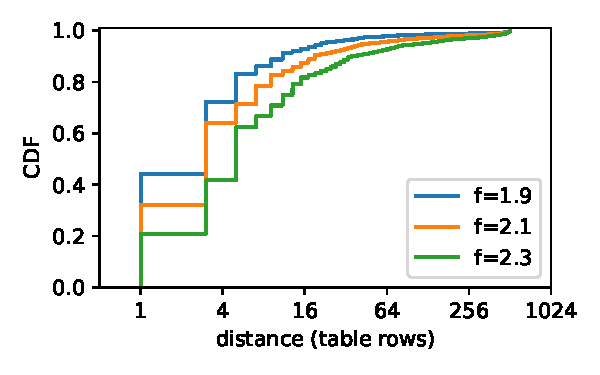
\includegraphics[width=0.99\linewidth]{fig/hash_factor.pdf}
        % \label{fig:hash_factor}
        % \caption{}
    \end{subfigure}
    \begin{subfigure}{0.3\linewidth}
        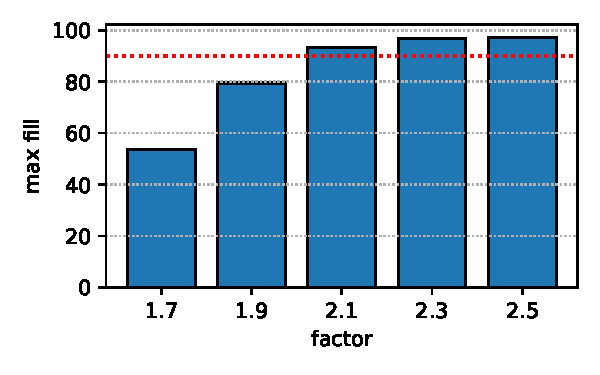
\includegraphics[width=0.99\linewidth]{fig/hash_fill.pdf}
        % \label{fig:hash_fill}
        % \caption{}
    \end{subfigure}.
    \vspace{-1em}
    \caption{
    \textbf{(a)} Dependent hashing for factor $f$.
    \textbf{(b)} CDF of distances between cuckoo locations dependent hashing on different exponential factors.
    \textbf{(c)} Exponential factor relation to max fill in cuckoo hash. 90\% fill marked in red.
    }
    \label{fig:locality-hashing}

\end{figure*}




\subsection{Dependent Hashing}

Cuckoo and hopscotch hashes are optimized for
reads~\cite{cuckoo,hopscotch} and have been used extensively
in RDMA key value
stores~\cite{memc3,cuckoo-improvements,pilaf,farm}. Both
hashes are read optimized, cuckoo hashing ensures at most
two reads are required (both can be done in parallel), while
hopscotch hashing ensures the locality of a read to a
specific location.

Our approach aims to combine the constant time reads of
cuckoo hashing with the locality properties of hopscotch
hashing. Traditional cuckoo hashing requires two independent
hash functions which set key locations uniformly at random.
We use two ~\textit{dependent} hash functions to increase
locality between key locations. The first hash function
selects a row in the cuckoo table uniformly at random. The
second second hash function selects a location randomly from
the following $n$ rows after the first hash location. The
value of $n$ is not constant. A third hash function $h_3(x)$
generates values of $n$ according to an exponential
distribution. We use a constant factor $f$ to control the
exponential function.  Figure~\ref{fig:locality-hashing}(a)
shows the formula for our dependent hash functions.

The constant value $f$ determines the distribution of
distances between key locations.
Figure~\ref{fig:locality-hashing}(b) is a CDF of distances
between key locations for 3 values of $f$. A distance of 1
means that a keys second location is in the row immediately
after it's first location. In the case of $f$=2.3 20\% of
keys have a distance of 1 bucket. Small values of $f$ have
high locality. However, locality is not free. Independent%%
hash functions enable cuckoo hashes to read high fill rates (95\% and higher).
%%
Removing independence increase the probability of
hotspots which cause insert operations to fail. A cuckoo
insertion fails if no sequence of swaps exists which can
produce a valid cuckoo path. Failed insertions require the
table to be resized and directly effect memory utilization.
Therefore $f$ is directly related to the maximum fill factor
a table can achieve using dependent hashing.

% An over
% filled region of the table can quickly lead to deadlocks
% when inserting requiring the table to be resized. $f$ is
% directly related to the max fill factor of the table. Larger
% $f$ values increase the max fill factor, while decreasing
% locality.  

Figure~\ref{fig:locality-hashing}(c) shows the relationship
between $f$ and a tables maximum fill. These values were
generated by inserting into a cuckoo table with 100M entries
until an insertion failed. Table associativity directly
effects fill rate. The higher the degree of associativity
the more likely a valid path will exist. The table used in
Figure~\ref{fig:locality-hashing} has an associativity of 8
similar to prior cuckoo
hashes~\cite{memc3,cuckoo-improvements,pilaf}.


% The associativity of the
% cuckoo hash plays a key role in enabling high fill. The
% higher the degree of associativity the greater degrees of
% freedom search is given to escape local hotspots.

%The second hash function determines the maximum
%distance the second value can have from the first. A third
%hash function determines a random location between the first
%location, and the bound imposed by the second.
% Figure~\ref{fig:locality-hashing}(a) shows the formula for our hashing
% function process, which implements the probabilistic region-size
% selection with a third hash function---akin to the way Bitcoin
% computes its difficulty.
% \textbf{Why not make the second hash function a true expoential?}

% A strawman implementation of locality based hashing would
% use the first hash function to find a location, and the
% second to find a random location within a fixed bound. This
% approach quickly leads to failed insertions. Due to the
% birthday paradox the probability of a collision is high, and
% on large tables the probability that one region of the hash
% table will become full, and have not viable path to an open
% slot is high. ~\sg{Perhaps this justifies a figure, please
% advise.}.

% We use a dynamic exponential bound rather than a static one.
% The dynamic bound is set by raising a constant factor $f$ by
% an exponent determined by a third hash function. Using the
% third hash on the key we count the number of suffix zeros
% and raise the constant factor by itself plus the zero count.
% This distribution generates exponential distances between
% hash locations at exponentially less frequency and is
% tunable with the single parameter $f$.
% %%
% In the common case the bound is small. Exponentially few key
% are spaced far apart and act as~\textit{waypoints} to other
% regions of the table when constructing cuckoo paths. This
% method, paired with bucket associativity enables high fill
% rates while keeping the region of the table any given key
% can inhabit small.

% There is a tradeoff between locality and fill factor.
% Figure~\ref{fig:locality-hashing}(b) illustrates how
% increasing the exponential factor shifts the distribution of
% distances between cuckoo hash locations.
% Figure~\ref{fig:locality-hashing}(c) shows how these same
% factors effect the max fill rate of the table before an item
% cannot be inserted. As will be shown in the following
% sections read, and insert performance improve with better
% locality. Therefore fill factor and performance can be
% traded off directly by changing the exponential factor. In
% our evaluation we found an exponential factor of 2.3 to give
% the best results in terms of end to end performance and
% bandwidth consumption.


\subsection{Locking}

\begin{figure*}[t]
    \centering
    \begin{subfigure}{0.3\linewidth}
        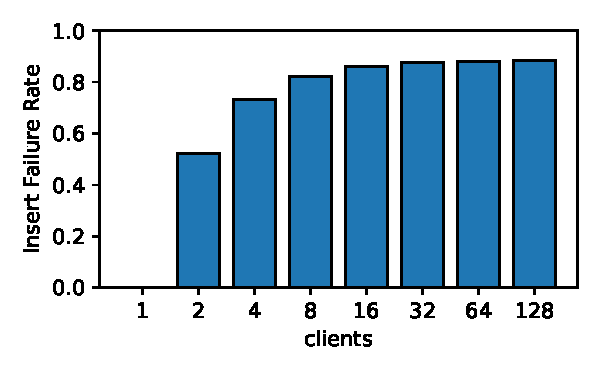
\includegraphics[width=0.99\linewidth]{fig/optimistic_failures.pdf}
        % \label{fig:optimistic_failures}
        % \caption{}
    \end{subfigure}
    \begin{subfigure}{0.3\linewidth}
        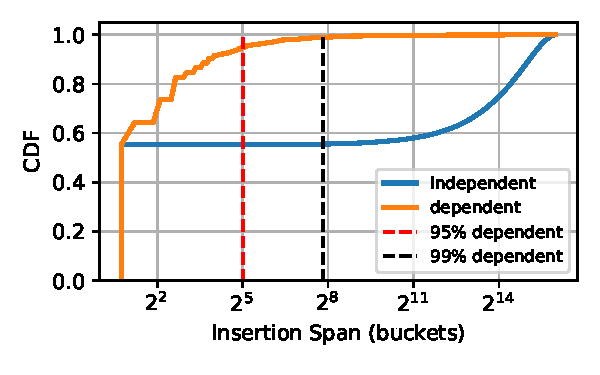
\includegraphics[width=0.99\linewidth]{fig/insertion_span.pdf}
        \label{fig:insertion_span}
        % \caption{}
    \end{subfigure}.
    \begin{subfigure}{0.3\linewidth}
        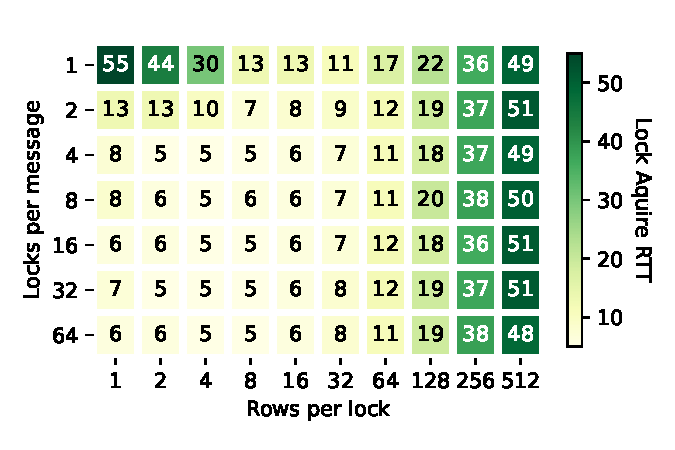
\includegraphics[width=0.99\linewidth]{fig/buckets_per_lock_vs_locks_per_message.pdf}
        \label{fig:tbd}
        % \caption{}
    \end{subfigure}.
    \vspace{-1em}
    \caption{
    \textbf{(a)} Failure rate of optimistic cuckoo insertions.
    \textbf{(b)} CDF of cuckoo spans for dependent and independent hashing. A cuckoo span is the distance between the smallest and largest index in a cuckoo path.
    \textbf{(c)} Round trips (99th percentile) required per insert while filling a table to 100\% while varying the lock per message, and buckets per lock. \todo{subtract one from each current values include unlocks}
    }
    \label{fig:cuckoo-problems}

\end{figure*}

Rcuckoo uses locks rather than optimistic operations
(compare-and-swap) so table entries can be larger than 64
bits. This enables fast reads, as both keys, and values can
reside directly in the table index. Locking can be
expensive, as a naive deadlock free aquire and release
protocol can incur many round trips.  in this section we
describe our lock table, and locking protocol designed to
achieve fast locking in an average of two round trips.

Our lock table is an array of contiguous bits where each bit
is a lock, and each lock guards one or more sequential
buckets. The size of the lock table in bytes equals the
number of hash table rows, divided by the number of rows
each lock guards (rows per lock). The size of a lock table
for a cuckoo table with 100M entries, 8 entries per row, and
16 rows per lock is 102KB.  Lock table size, and rows per
lock are important variables as they enable us to utilize
two features of modern RDMA NICs, mainly device mapped
memory, and masked compare and
swap~\cite{rdma-masked-cas,sherman}.

Device mapped memory is a small reigon of on NIC memory,
typically on the order of 256KB. This memory executes
one-sided RDMA operations faster than host memory as the
operations need not make a PCIe round trip. This memory is
especially performant for atomic operations as the NIC would
otherwise have to queue dependent atomic request to host
memory. Figure~\ref{fig:rdma-benchmarks}(c) shows the
performance boost from device over host memory for atomic
operations.

The second NIC feature we exploit is masked compare and swap
operations ~\ref{fig:rdma-masked-cas}. Masked cas operations
enable clients to set individual bits rather than 64 bit
spans. As our lock table is tightly packed this enables
clients to aquire locks without any additional knowledge
about the lock table as would be required for unmasked cas.

Together with locality hashing these features enable the
following fast locking protocol. When a client requires
locks it calculates all lock indexes locally. Lock indexes
are the row the client must lock divided by the number of
rows per lock. Once the set of locks is calculated the
client breaks the set of locks into separate locking
requests. If the locks are within 64 entries of each other
all locks are packed into a single masked compare and swap
packet. If the span of locks is greater than 64 a second
packet is generated with all locks in the next range of 64
packed together into a single packet. To avoid deadlocks
lock request are issued one at a time. Clients repeatedly
request the same locks until they are acquired. Lock
releases are done in a single batch.

% We use RDMA device memory for our lock
% table~\cite{rdma-masked-cas}. To aquire locks clients
% locally determine which locks they require for their
% operation, and then issue RDMA masked CAS operations to the
% device memory. This approach enable clients to aquire up to
% 64 contiguous locks with a single RDMA operation and enable
% clients to aquire locks without synchronizing the state of
% the lock table prior to acquisition (non masked CAS would
% need the state of all locks prior to issuing the request.).

This locking scheme in conjunction with dependent hashing
enables most client operations to aquire locks in a singe
round trip. Update and insert operations require at most two
locks, one for each key location. Using $f$ of 2.3 90\% of
key pairs are within 64 rows of each other so even with row
per lock 90\% of updates and deletes can be completed in two
round trips. In practice we use 16 rows per lock which
results in 99.7\% of updates and deletes resulting in two
round trips.

Inserts can span arbitrary regions of the table and are a
harder case than updates and deletes.
Figure~\ref{fig:cuckoo-problems}(b) shows the span in rows
of cuckoo paths for a table with 100K rows. These spans are
the difference between the highest and lowest row locked
during insertion. Using dependent hashing 95\% of insertions
span 32 rows or less, and 99\% of insertions span 256 rows
or less. Using 16 rows per lock each masked cas can cover
1024 rows of the table ensuring that 99.5\% of insertion
locks can be acquired in a single round trip.

% Using this locking scheme locality hashing greatly improves
% locking performance. With independent hashing the locks for
% a cuckoo path are scattered randomly throughout the table.
% Therefore, a round trip is required for each lock, and each
% lock must be acquired in order to avoid deadlock. With
% locality, and the ability to lock up to 64 sequential locks
% most insertions can be performed with a single round trip
% for locking. In both cases lock release can be batched in a
% single round trip.

% Figure~\ref{fig:cuckoo-problems}(b) shows the insert span in
% buckets using both dependent and independent hashing on a
% table with 500K entries and an associativity of 8. A span is
% calculated as the distance between the lowest index and the
% highest index in a cuckoo path. Past 50\% independent
% hashing spans a random range in the table (whenever a
% displacement occurs on insert). With dependent locality
% based hashing 95\% of inserts span less than 32 buckets, and
% 99\% less than 256.


% Traditional wisdom would suggest that because cuckoo hashing
% can have long insertion paths it is a poor candidate for
% remote memory. Both opportunistic, and lock based approaches
% have significant drawbacks.
% %%
% As an example consider an opportunistic approach in which
% many clients are inserting concurrently to a table. Clients
% making inserts first make reads of the table to locally
% calculate a cuckoo path for their insertion. After the reads
% complete the client constructs a cuckoo path and starting
% from the open slot issues dependent CAS requests migrating
% the open slot backwards to the insertion bucket.
% %%
% Figure~\ref{fig:cuckoo-problems}(a) shows the failure rate
% of this insertion scheme as a factor of clients running
% inserts on a table with 500K entries with a bucket
% associativity 8. Cuckoo paths calculated from client caches
% quickly become invalid as the number of clients grows.
% %%
% Alternatively deadlock free lock acquisition requires more
% round trips and has larger critical sections. Each lock must
% be acquired in order with a dependent CAS request which
% incurs an additional round trip per lock. Using course
% grained locks reduces the number of acquisitions but
% throttles throughput as concurrent insertions are more
% likely to contend shared locks.

% Locality hashing increases the probability that an insertion
% path is within a small region of the hash table which in
% turn increases the probability that fine grained locks will
% be near one another. 
% %%
% Figure~\ref{fig:cuckoo-problems}(b) shows the insert span in
% buckets using both dependent and independent hashing on a
% table with 500K entries and an associativity of 8. A span is
% calculated as the distance between the lowest index and the
% highest index in a cuckoo path. Past 50\% independent
% hashing spans a random range in the table (whenever a
% displacement occurs on insert). With dependent locality
% based hashing 95\% of inserts span less than 32 buckets, and
% 99\% less than 256.
% %%
% RDMA masked CAS operations allow a client to set a 64 bit
% mask along with the new, and old values of the cas
% operation. So locks can be acquired with minimal knowledge
% of the remote lock table. This enables the client to
% atomically set up to 64 contiguous locks independently which
% dramatically reduces the round trips required to aquire
% locks.

% Lock granularity effects performance under contention. Using
% values from Figure~\ref{fig:cuckoo-problems}(b) if locks are
% per bucket 96\% of lock acquisitions can be completed with a
% single RTT masked cas. If locks span 4 buckets 99\% of
% requests can be completed in a single round trip.

% Increasing the number of buckets each lock guards can reduce
% the number of locks required for an operation.
% Figure~\ref{fig:ycsb_fill_latency}(c) shows the tradeoff
% between lock granularity and the number of locks which can
% be set in a single message with locality hashing turned on.
% The table has 512 rows total to illustrate the effect of a
% single global lock.

% The values
% reported are the 99th percentile number of round trips
% required to acquire locks up to a 90\% fill factor on a
% table with 4096 entries and 8 entries per bucket, and 8
% concurrent clients. The biggest factor in round trip times
% is the number of locks per bucket. On the far right side of
% the heatmap (512) only a single global lock exists. Further
% the benefit in terms of locks per message falls off quickly
% after two. RDMA-masked CAS are beneficial as they allow for
% fine-grained locking, but setting 3 or more locks per
% message has little effect up to 90\% fill rate. Reducing
% atomic operations in turn reduces the effect of the RDMA
% atomic bottleneck.  \textbf{Hard to see 3; the figure only shows 2 or 4.}

% Our lock table is small in comparison to the true hash
% table. At its most fine-grained each lock corresponds to
% one bucket (8 entries). Each lock is 1 bit, a lock table for
% a 100 million entry hash table is ~160KB, with a lock
% granularity of 4 buckets this drops to 40KB. This tight
% layout enables us to use device-mapped memory to hold our
% lock table~\cite{design-guidelines,sherman}.
% %We make use of
% Device-mapped memory on recent RDMA NIC's (ConnectX-5+) avoids an
% expensive PCIe round trip, reducing lock acquisition latency.
% This enables up
% to 3$\times$ better throughput on contested locks (see
% Figure~\ref{fig:rdma-benchmarks}(c)), and reduces latency
% for locking.

\subsection{Table Design}

\sg{@alex I've left the proposed table design in}

We design our hash table for fast reads as most data center
key-value workload are read heavy~\cite{facebook-workloads}.
Prior disaggregated indexes such as
~\cite{clover,race,fusee} require two round trips minimum
for first time reads as their indexes do not support
inlining. In the case of RACE and FUSEE index entries are
fixed to 64 bits to support RDMA CAS width operations. This
fact prevents both projects from inlining key value data and
requires them to make a second round trip to an extent to
retrieve data, and check if a key is present in the table.

In our table users can specify the size of their index entries at
initialization time. Key value pairs which are small enough
to fit within the index are inlined, otherwise they are
stored in an extent. Figure~\ref{fig:table-diagram}
illustrates our table design. Each entry includes an extent
bit to indicate if the entry is inlined or stored in an
extent.

\subsubsection{Client Caching}

\todo{expand} Clients cache duplicates of the remote index
to improve the performance of operations. In the case of
insertions clients search their locally cached indexes to
determine a cuckoo path prior to acquiring locks. 

\subsubsection{Memory Allocation}

Prior work has focused on different memory allocation and
hash table resizing schemes. Sherman~\cite{sherman} uses an
allocated thread located on the memory node,
Fusee~\cite{fusee} uses a two tired memory allocation in
which large blocks of memory are allocated on the memory
nodes and fine grained allocation is performed on the
clients. Clover~\cite{clover} statically partitions memory
into large client regions prior to execution and hash
clients entirely manage the space themselves. Network based
allocators such as MIND and Clio~\cite{mind,clio} have
demonstrated the feasibility of high performance
disaggregated allocators, while some have called for
allocators to be built into RDMA~\cite{prism}. We allocate
memory using the same scheme as Clover, as it is simple to
implement and adds no additional overhead. We view memory
allocation as a hard orthogonal problem to the design of
disaggregated indexes and have designed our system
acrostically to the allocator.




\begin{figure}[t]
    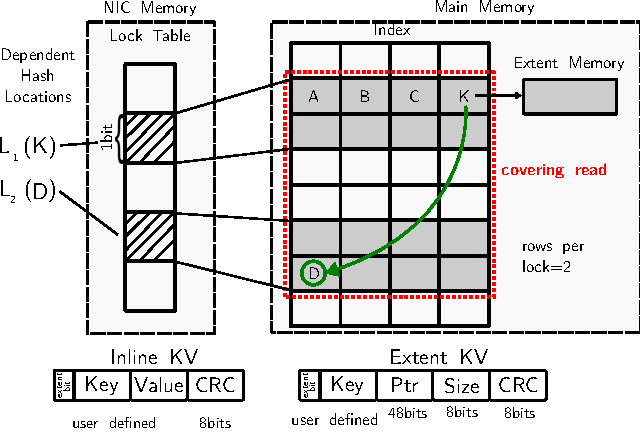
\includegraphics[width=0.99\linewidth]{fig/table-diagram.pdf}
    \caption{Rcuckoo's table design ~\todo{remove extents for this submission}}
    \label{fig:table-diagram}
\end{figure}


\subsection{Protocol}

\begin{figure}[t]
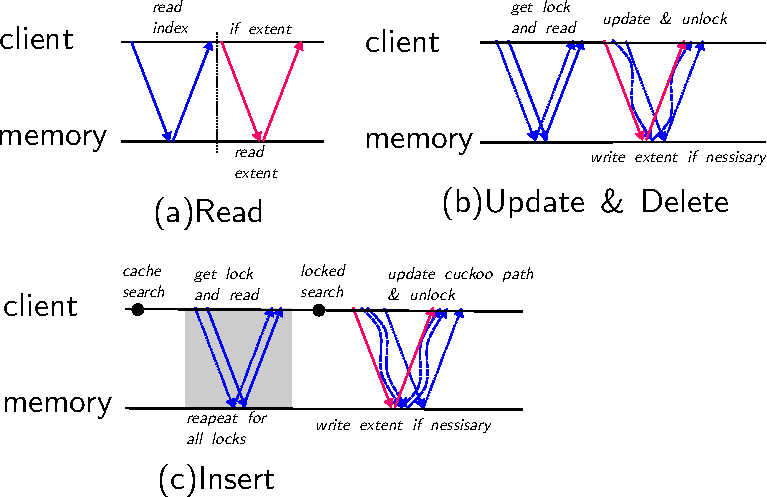
\includegraphics[width=0.99\linewidth]{fig/message_diagram.pdf}

\caption{Rcuckoo's protocol for reads, inserts, deletes and
updates. Blue lines are index accesses, and red lines are
extent accesses. Solid lines are reads, dotted lines are
CAS, and curved dashed lines are writes.}

\label{fig:message_diagram}
\end{figure}

In this section we describe our protocol for reading,
inserting, and performing updates and deletes to an rcuckoo
hash table. Figure~\ref{fig:message_diagram} visualizes our
protocol.

\subsubsection{Reading} 
\label{sec:reading}

Client read request are closely similar to traditional
cuckoo hashing with two additional performance
optimizations. To read a key $k$ clients first locate both
key locations. In default cuckoo hashing two reads are
issued in parallel to both rows. We take advantage of
dependent hashing locality and issue a single read which
captures both rows if the distance between key locations is
less than a predefined threshold. If key locations are in
adjacent rows a single read saves packet processing time,
network bandwidth due to header size, and waiting time as
the client need not wait for a second read to return. Larger
reads consume additional bandwidth but still provide some
additional performance (see Section~\ref{sec:read-threshold}).

If key-value entries are inlined reads complete in a single
round trip. Larger key stored in extents require a second
round trip as clients must first read the index, resolve the
virtual address of the extent and then perform the extent
read.
%%
~\footnote{This design requires exactly one pointer
resolution in expectation that future RDMA NICs may provide
pointer resolution reads as a primitive~\cite{prism}}
%%
As reads are lockless they can occur simultaneously with
writes updating the table. Each entry contains a CRC which
is checked on reads to validate that all writes have
completed~\cite{pilaf,cell}.
%%
We define a read threshold of 512 bytes for our clients.
Approximately 60\% of keys for 64-bit entries with a bucket
size of 8 (see Figure~\ref{fig:locality-hashing}(b)) fall
into this category. This has the advantage of updating the
client cache for future operations.
%, and reduces the header processing required by the NIC.
To reduce bandwidth the size of the threshold can be tuned
down, or turned off with no harm to correctness.

% \subsubsection{Locking and unlocking}

% Update, delete and insertion operations all require locks to
% modify the index. Locks are acquired in incremental order
% from smallest to largest to avoid deadlocks. First the list
% of locks required for the operation is calculated. For
% updates and deletes two locks may be required. Inserts may
% required many locks. The client calculates which locks it
% requires and breaks the list into masked CAS operations
% spanning 64 locks and then issued the requests polling for a
% successful response before moving to the next lock.

% To synchronize the client cache with remote memory we issue
% a \textit{covering read}. A covering read is an RDMA read
% which spans the range of buckets from the lowest lock in the
% masked CAS to the highest. The covering read is issued after
% the masked CAS and ensures the client receives synchronized
% data for the locked buckets while not consuming an
% additional round trip.

% Clients need their caches synchronized with remote memory
% prior to modifying it with writes. We batch reads with lock
% requests to synchronize client caches. RDMA in-order
% delivery ensures that reads issued after a lock request will
% be up to date, as no other client can concurrently modify
% the locked index.  A spanning read is issued for each lock
% request. The read covers each bucket the client locks.  For example, if a
% masked CAS has three locks, reads are calculated for each
% bucket being locked. If the locks cover a range less than
% the read threshold a single read is issued which spans all
% buckets between the locks.  Spanning reads are issued concurrently with
% lock requests.
%Subsequent lock requests are issued prior to
%blocking on reads.

% After locks are acquired the client can execute its critical
% section. Unlock requests are the inverse masked CAS operations of the
% lock requests. Clients issue their critical sections as a sequence of
% (asynchronous) writes followed immediately by unlock operations. RDMA
% in-order delivery ensures that the unlock operations are performed
% after the writes.

\subsubsection{Updates and Deletes}

Updates and deletes are similar operations as both require
two locks. In the locking phase clients calculate and aquire
both locks~\ref{sec:locking}. Updates to inlined entries
issue a single entry sized update directly to the index.
Updates to extents issue three messages first the new extent
is written, the index is updated, and finally the old extend
is set to invalid and marked for garbage collection. In both
cases unlock messages are batched with the update. Similarly
deletes lock both table entries. On deletes clients compact
the row so open entries are always located at the end of the
row~\footnote{Ensuring open entries are at the ends of rows
improves search times for open buckets.}. Extent entries are
marked as invalid in the same round trip. Both updates and
deletes commonly execute in 2 round trips. 3 round trips are
required only if both locks are too far apart to be set in a
single masked cas operation.

\subsubsection{Insert}

Unlike updates and deletes, inserts may require modifying
locations spread across remote memory and require many
locks. The main challenge in performing an insert is
determining which locks to aquire. A naive approach would
use a global lock, or incrementally aquire locks during
search. These approaches are known to throttle throughput,
and require many round trips to
complete~\cite{cuckoo-improvements}. Unlike prior work,
issuing reads to the remote index while searching is
untenable as it will frequently require many round trips to
build a cuckoo path.

We design a novel two stage search approach to minimize
round trips while producing valid cuckoo paths with high
probability.

\textbf{Speculative Local Search:} The first stage of
insertions is a speculative local search. Clients calculate
an cuckoo path by searching their unsynchronized local
caches. While This may not produce a valid cuckoo path it
constructs a speculative cuckoo path which is localized to
the region of the table likely to contain a vaild path. When
the table hash low fill, the speculative path is frequently
correct. Using the speculative path, the client calculates
the locks required for the speculative insertion aquire the
unessisary locks.

Clients synchronize their caches during lock acquisition.
Using the speculative path, clients use a \textit{covering
read} which spans the locked rows. As covering reads can be
large we limit them to the same size as the read threshold.
Covering reads are batched together with lock requests but
are sequenced after. As such the values returned by the read
after a successful lock aquire are fully synchronized.

\textbf{Second Search:} The speculative path may not be
valid after clients have acquired locks and synchronized
their caches. If the speculative path is not valid clients
perform a second search restricted to the rows locked by the
client. Due to dependent hashing cuckoo paths are highly
localized. If locks cover 8 or more rows clients have a high
probability of constructing a valid cuckoo path using the
rows locked by their first search. If clients can not find a
valid path with their second search the client releases it's
locks and tries again. Subsequent searches have a high
likely hood of success as clients retain their caches across
requests. We measure the success rate of second searches in
response to the number of rows per lock in our evaluation
section~\ref{sec:second-search}.

Cuckoo paths and updates are issued in a single batch. If a
valid search path is found path updates are made as a batch
of sequential writes. Unlock operation are batched after the
writes. Writes to the extent precede updates to the table.

Insertions are the most expensive operation as they require
computation, large reads, and writes. In our evaluation we
find that insertions are limited by the network bandwidth of
our CX5 NIC's not lock contention or failed searches. We
consider this a desirable limitation as network bandwidths
continue to increase and so additional operation throughput
can be exchanged for additional bandwidth~\footnote{CX7
NIC's currently support 400Gbps line rate.}.

% Clients must first aquire
% remote locks and then synchronize their cache before they
% can calculate a guaranteed valid cuckoo path. Acquiring many
% locks speculatively can decrease throughput by blocking
% concurrent clients. Simultaneously performing huge
% synchronizing reads can absorb unessisary bandwidth.


% Determining which locks to aquire is hard as clients
% may have stale caches and many options for potential
% insertions paths.  We use a speculative two-phase search
% strategy to find and execute insertions with high
% probability in two rounds trips. First the client searches
% it's local cache for a potential cuckoo path. Once a path is
% found the client calculates the set of locks it requires and
% attempts to aquire the locks for the speculative cuckoo
% path. As locks are speculative reads synchronize the client
% cache.

% After the speculative locks are acquired the client performs
% a second search only using the locked buckets in the table.
% If no such path can be found, the client releases the locks
% and tries again. If a new path can be found using the locked
% buckets that path is executed and the lock is released.
% This search strategy benefits greatly from course grained
% locks. We have found in practice that setting each lock to
% cover 8 buckets yields the highest performance. Given the
% distribution of the locality hash function there is high
% probability that an insertion path can be found within the
% 64 locked buckets. In the common case this means that
% inserts take only two round trips. On failures the client
% maintains the cache it built during the first search to
% improve its chances of finding a path on the next attempt.


% We use a two-phase search
% strategy to find insertion paths. First the client
% constructs a potential cuckoo path using its cached index.
% The client then attempts to acquire the locks necessary for
% its cuckoo path. Thanks to the spanning reads, once a client
% succeeds in acquring the necessary locks its cache has been
% fully synchronized with the relevant portions of remote
% memory. A second search is then performed using only the
% buckets the client succeeded in locking---which may be the
% same if the client's cache was completely up to date. If
% this search is successful the client calculates the updates
% to the cuckoo path batches them as a series of writes and
% issues them along with it's unlock requests.

% If the first search fails the client performs a read and
% tries again. If this fails the table must be resized. The
% second search may fail because the clients cache was stale
% and the list of locked buckets was insufficient to perform
% the insert. In this case the client releases the locks and
% performs the insertion from the start again by performing an
% unrestricted search on its local cache. In the common case
% insertions take two round trips: We find that when the table is less
% than 50\% full the probability that a cuckoo path has
% length greater than one is low. If extents are
% used the client batches the extent write during its locking
% phase.

% \textbf{Key Duplication:} Unlike RACE our algorithm can
% prevent duplicate keys easily on insert~\cite{race}. RACE
% requires three round trips for inserts, the third re-reads
% the index to ensure no duplicates were inserted
% concurrently.  Alternatively Cuckoo hashing inserts to
% exactly one bucket, which is read during the lock
% acquisition phase. If a duplicate key is found the client
% can abort. If the bucket is full, a duplicate key may exist
% in itts alternative bucket. Our clients issue a read to the
% inserted keys alternative bucket during lock acquisition. If
% the lock returns successfully and no duplicate exists in
% either bucket then no duplicates exist as the successful
% lock ensures that no other client is currently moving the
% key to another location as part of a concurrent insert.


\subsubsection{Search Algorithm} 

Cuckoo paths are highly influenced by the search algorithm 
used to find them. Prior work has used DFS to construct 
cuckoo paths~\cite{pilaf,memc3}. We follow prior work and 
use BFS as it produces the shortest 
paths~\cite{cuckoo-improvements}. Short paths reduce the 
number of locks required. Dependent hashing opens new 
opportunities for search optimization as open slots are more
likely to be close to an initial hash location. As part of
our work we investigated using guided search A* to construct
short paths using locality information. We found that A*'s
performance only improves on BFS at fill rates about 95\%
which are rarely found in practice due to max fill rate
limitations.

% Locality based hashing provides us opportunities for better
% search than traditional cuckoo hashing. Cuckoo hashing
% insert traditionally uses random replacement~\cite{cuckoo}.
% Random replacement requires little computation, however at
% high fill rates it leads to long cuckoo paths which require
% many locks, and reduce concurrent throughput. BFS search
% finds the shortest path and has been demonstrated to
% increase system throughput with fine-grained
% locking~\cite{cuckoo-improvements}.  BFS is computationally
% intensive. Locality based hashing enables us to leverage
% more efficient search strategies. Because locality hashing
% increases the probability that a cuckoo hashing location is
% close we can use an informed search algorithm to find open
% slots close to bucket a key hashes to. 
% %%
% In the case of BFS the target bucket is unknown, therefore
% all paths must be explored. We use A* search, an algorithm
% which takes a goal location, and a distance heuristic as
% input. A* is known to find shortest paths in much better
% average-case times than BFS~\cite{}. A* requires two
% additional inputs, a distance heuristic and a goal location.

% \textbf{Goal location}: Locality hashing increases the
% probability that an open slot near the insertion target
% location can terminate a cuckoo path. Our algorithm collects
% open slots near the original hash location as candidate goal
% locations. By default we set the number of candidate goal
% locations to 5. Goal locations are collected by starting at
% the $h_1(k)$ location and iterating through the hash
% table both forward and backwards through the table one index
% at a time. Buckets with open slots are added to the
% candidate list until the limit is reached. 

% \todo{I could
% improve this search time by tracking the list of open
% buckets and using binary search on them.}.

% \textbf{Search Heuristic}: A* requires a heuristic for
% distance which is a strict underestimate of the true
% distance to a goal. A typical heuristic for search is the
% euclidean distance between two points. A * guarantees that
% if the search heuristic is a strict underestimate of the
% true distance to the goal then the path found will be the
% shortest path. In our case we use the distance between a
% goal state and a current state is unknown as the distance
% between any two buckets is the result of our locality
% hashing function which has no upper bound. However we can
% estimate the distance between two buckets by using the mean
% distance of our locality hash function. This approach does
% not guarantee that we find the shortest path, however it
% does find short paths in the common case, and results in
% very short search times.

\subsection{Replication, and scalability} 

\todo{no real replication probabily delete, consider moving
to future work / limiations} At the time of writing RCuckoo
does not support replication although replication is in no
way a complication for our existing algorithms. On inserts
clients aquire locks from a master memory node as described
in section~\ref{sec:insert}, after locks are acquired on the
master node updates, deletes, or cuckoo paths are broadcast
to replicas. Replication requires a clients to wait for
responses from replicas before issuing unlock messages as
the client can not rely on RDMA RC connection in order
delivery across the multiple replica connections.

\todo{We don't span multiple memory nodes} When using
multiple memory machines each machine is initialized with an
equal portion of the cuckoo index and lock table. Clients
calculate which machine to issue their requests to when
generating requests.

